% !TeX root=../../../main.tex

\chapter{روش پیشنهادی}
%\thispagestyle{empty} 
\section{مقدمه} 
%پس از آشنایی با روش‌های پیشین که برای حل مسئله مشابه مورد استفاده قرار گرفته‌اند، حال می‌توانیم به معرفی و تشریح روش‌های پیشنهادی خود برای حل مسئله پیش رو بپردازیم. در این فصل ابتدا داده‌های ورودی مسئله را همراه با فرضیات در نظر گرفته شده بیان می‌کنیم و پس از آن دو روش پیشنهادی متفاوت را بیان خواهیم نمود. در روش اول که به رویکردهای پیشین نزدیک‌تر است با تغییری از جنس روش‌‌های نوین در مراحل میانی به یک روش جدید می‌رسیم که به علت افزایش سرعت همگرایی می‌توان فرض و داده‌های جدیدی را از طریق \gls{cnv} به آن افزود و پاسخ گرفت. اما روش دوم کاملا متفاوت بوده و با رویکردی جدید در حوزه یادگیری ماشین همراه است که به کمک یادگیری تقویتی به حل مسئله مورد نظر می‌پردازد.

پس از آشنایی با روش‌های پیشین که برای حل مسئله مشابه مورد استفاده قرار گرفته‌اند، حال می‌توانیم به معرفی و تشریح روش‌ پیشنهادی خود برای حل مسئله پیش رو بپردازیم. در این فصل ابتدا داده‌های ورودی مسئله را همراه با فرضیات در نظر گرفته شده بیان می‌کنیم و پس از آن روش پیشنهاد خود را بیان خواهیم نمود. این روش با الهام از ۳ روش قبلی متفاوت تنظیم شده است. در ابتدا پایه و بنیان آن به یکی از رویکردهای پیشین نزدیک‌تر است که با تغییری از جنس روش‌‌های نوین در مراحل میانی به یک روش جدید می‌رسیم که به علت افزایش سرعت همگرایی می‌توان فرض و داده‌های جدیدی را از طریق \gls{cnv} به آن افزود و پاسخ گرفت که این عمل با بهره‌گیری از رویکردی جدید در حوزه یادگیری ماشین همراه است که به کمک یادگیری تقویتی به حل مسئله مورد نظر می‌پردازد.

\section{معرفی دادگان ورودی}
قبل از وارد شدن به بخش روش‌های پیشنهادی نیاز است تا دادگان ورودی را مشخص و معرفی نماییم. دادگان ورودی در این پایان‌نامه همگی به صورت فایل‌های خام \gls{ascii} هستند که حاوی اطلاعات جهش‌های ماتریس ژن-سلول (\lr{SNV}) و اطلاعات مربوط به \gls{cnv} هستند.

در ادامه جدول
\ref{tab:ch_pm:firstpmIndices}
را برای معرفی اندیس‌های بکار گرفته شده در روابط مربوط به روش پیشنهادی اول معرفی می‌نماییم.

	\begin{table}[ht]
	\caption{اندیس‌های به کار رفته در روابط روش پیشنهادی اول}
	\label{tab:ch_pm:firstpmIndices}
	\centering
	\onehalfspacing
	\begin{tabularx}{0.9\textwidth}{|r|X|}
		\hline
		$D$	& ماتریس داده نویزی در دسترس که مقادیر $0$ و $1$ در آن قرار دارد \\
		\hline
		$E$	& ماتریس داده حقیقی بدون نویز که به دنبال آن هستیم \\
		\hline
		$T$	& درخت فیلوژنی جهش‌ها \\
		\hline
		$\sigma$	 & بردار انتصابات \\
		\hline
		$\wp$ & بردار پذیرش فقدان$  $ \\
		\hline
		$X_T$	& ماتریس متناظر درخت $T$ \\
		\hline
		$N$	& تعداد سلول‌های نمونه \\
		\hline
		$M$	& تعداد جهش‌ها \\
		\hline
		$\mathcal{N}$ & مجموعه سلول‌های متمایز از هم \\
		\hline
		$\mathcal{M}$ & مجموعه جهش‌های متمایز از هم \\
		\hline
		$\mathcal{L}$ & مجموعه جهش‌های با پتانسیل حذف \\
		\hline
		$\alpha$	&  نرخ خطای \gls{falsepositive} \\
		\hline
		$\beta$	& نرخ خطای \gls{falsenegative} \\
		\hline
	\end{tabularx}
\end{table}



\section{روش پیشنهادی برای مدیریت داده‌های از دست رفته}

در ادامه این بخش به معرفی روش‌های پیشنهادی پرداخته خواهد شد اما در ابتدا به دلیل وجود داده‌های از دست رفته در پایگاه‌داده‌های مورد استفاده لازم است تا به بررسی و ارائه رویکردی برای حل این مشکل پرداخته شود و در ادامه پس از معرفی روش پیشنهادی برای مددریت این داده‌های از دست رفته، هر کدام از روش‌های پیشنهادی به تفضیل شرح داده شود.

همان‌گونه که در داده‌های حقیقی مشاهده شد در پایگاه داده‌های حقیقی ما با اطلاعات از دست رفته مواجه هستیم و به همین دلیل نیز سعی کردیم تا در پایگاه داده مجازی تولید شده نیز به مشابه داده‌های حقیقی، شامل اطلاعات از دست رفته باشد. در این بخش به رویکرد روش محاسبه استاتیک برای مدیریت این داده‌های از دست رفته می‌پردازیم و در بخش بعد به معرفی روشی برای بدست آوردن درخت فیلوژنی پرداخته خواهد شد. همان‌گونه که در ادامه بررسی خواهد شد، این اطلاعات از دست رفته در پایگاه داده‌های مختلف نرخ‌های متفاوتی دارد که تاثیر این تغییرات نیز در روشی پیشنهادی بررسی خواهد شد.

\subsection{روش محاسبه استاتیک}
در این روش قصد داریم تا به یک‌باره بتوانیم مقادیر مناسب برای داده‌هایی که از دست رفته‌اند را تخمین بزنیم. در این روش باید توجه شود که ما لزوما به دنبال جایگذاری مقدار از دست رفته با مقدار درست واقعی نیستیم. اگرچه چنین بیانی در نگاه اول ممکن است تعجب‌آور باشد اما با دقت بیشتر متوجه خواهیم شد که ما در آینده برای خطاهای موجود در پایگاه داده مدل‌سازی‌های محدودی داریم. مدل‌هایی که بهترین آن‌ها نیز ممکن است با واقعیت نویز افزوده شده به دادگان متفاوت باشد. در نتیجه اگر مطمئن بودیم که تمام داده‌هایی که موجود می‌باشند بدون خطا هستند در آن صورت ما نیز به دنبال یافتن جایگذاری با مقدار واقعی بودیم اما در حال حاضر که درصدی از داده‌های در دسترس خود همراه با خطا می‌باشند، ما به دنبال جایگذاری‌ای هستیم که بتواند در مجموع با مدل‌سازی خطایی که در نظر می‌گیریم بیشترین سازگاری را داشته باشد کما اینکه ممکن است در حقیقت جایگزاری اشتباهی انجام داده باشیم. حال با توجه به توضیحی که بیان شد به تشریح این روش می‌پردازیم.

با توجه به فرض مدل مکان‌های بی‌نهایت می‌دانیم که جهش‌های اتفاق افتاده در والد در تمامی نسل‌های آینده باقی خواهد ماند. بنابرین اگر تمامی جهش‌های نمونه (سلول) $a$ در نمونه‌ای دیگر مانند $b$ قرار داشته باشد، بنابرین می‌توان نتیجه گرفت که $a$ یکی از اجداد $b$ خواهد بود. همین فرضیه هسته اصلی روش پیشنهادی درنظر گرفته شده را تشکیل می‌دهد. بنابرین اگر جهش $i$ در سلول $a$ از دست رفته است، با توجه به اینکه آن جهش در سلول $b$ چه وضعیتی دارد می‌توان تصمیم‌گیری کرد. اگر $b(i)=0$ باشد، در این صورت $a(i)$ حتما باید $0$ باشد وگرنه فرض اولیه مدل مکان‌های بی‌نهایت نقض خواهد شد. اما اگر $b(i)=1$ باشد، آنگاه نتیجه خاصی نمی‌توان گرفت و باید به دنبال نمونه والد $a$ یعنی نمونه $d$ باشیم. حال اگر $d(i)=1$ باشد، آنگاه $a(i)$ حتما باید $1$ باشد. اما اگر $d(i)=0$ بود آنگاه انتخاب هر مقداری برای $a(i)$ تقریبا آزاد خواهد بود زیرا با فرض اولیه تناقضی ندارد و اینکه ساختار فیلوژنی را تغییر نمی‌دهد. اما از آنجایی که  خود داده‌های در دسترس شامل خطا می‌باشند و هر نمونه‌ای که حاوی اطلاعات از دست رفته است لزوما یک نواده یا یک والد ندارد، مجموعه‌ای از سلول‌های فرزند یا والد خواهند بود که متناسب با پارمترهای خطایی که در نظر می‌گیریم و فاصله ژنی‌ای که دارند می‌توانند در تصمیم‌گیری تاثیرگزار باشند. صورت دقیق‌تر توضیحات داده شده را می‌توان به صورت فرمولی که در ادامه آمده است به نمایش درآورد.
\\
در ابتدا تابعی به نام $F_s(D_{ij})$ تعریف می‌کنیم که به نوعی با توجه به ارزشی که به سلول‌های نواده شده از سلول $j$ می‌دهد سعی دارد تا اطمینان $0$ بودن داده از دست رفته $D_{ij}$ را بیان کند.
\\
برای محاسبه این تابع می‌دانیم که ابتدا سلول‌های مختلف با توجه به احتمال نواده بودنشان باید رتبه‌بندی شوند و وزن بگیرند. پس از آن  هر سلول متناسب با ارزش تاثیرگزاری خود می‌تواند در مورد جایگاه جهش $i$ برای سلول $j$ نظر دهد.
\begin{equation}
	F_s(D_{ij}) = \sum_{n \in \mathcal{N}}  (1-D_{mj})  \prod_{m=1}^{M} W(D_{mn}, D_{mj})
	\label{eq:ch_pm:F_s_simple}
\end{equation}

در فرمول \ref{eq:ch_pm:F_s_simple} مجموعه $\mathcal{N}$ برابر با مجموعه سلول‌های متمایز از هم است. زیرا که در بسیاری از پایگاه‌داده‌ها از یک نمونه سلول ممکن است چندین نمونه وجود داشته باشد که وجود آن‌ها باعث بایس در محاسبات ما خواهد شد. همچنین تابع $W_s(c,p)$ به ارزش‌دهی جهش $c$ در برابر $p$ به عنوان نواده بودن می‌پردازد که در فرمول \ref{eq:ch_pm:W_simple} تعریف شده است.
\begin{equation}
	W(c, p) = 
	\begin{cases}
		1 	       &\qquad \text{\lr{if}} \quad c=1, p=1 \\
		1-\xi   &\qquad \text{\lr{if}} \quad c=1, p=0 \\
		0 		  &\qquad \text{\lr{if}} \quad c=0, p=1 \\
		1 	 	  &\qquad \text{\lr{if}} \quad c=0, p=0
	\end{cases}
	\label{eq:ch_pm:W_simple}
\end{equation}
مقدار $\xi$ عددی بین $(0,1)$ است که پارامتری در جهت میزان ارزش‌دهی به نوادگان با فواصل مختلف می‌باشد. هرچه این عدد بزرگتر باشد به معنی کم‌ارزش‌تر شدن نوادگان با فواصل بیشتر است و بلاعکس.
\\
به همین صورت برای اولاد سلول $j$ نیز می‌توان مشابه حالت قبل عمل کرد که روابط آن به صورت فرمول‌ \ref{eq:ch_pm:F_a_simple} خواهد شد.
\begin{equation}
	F_a(D_{ij}) = \sum_{n \in \mathcal{N}}  D_{mj}  \prod_{m=1}^{M} W(D_{mj}, D_{mn})
	\label{eq:ch_pm:F_a_simple}
\end{equation}
حال دو نکته در استفاده از روابط بالا باقی خواهد ماند. 
\\
نکته اول وجود داده‌های دیگر از دست رفته در محاسبه توابع است که به دو صورت می‌توان با آن‌ها برخورد  نمود. رویکرد اول این است که در آن‌جایگاه ژنی از محاسبه آن خود داری شود و رویکرد دوم استفاده از از مقدار $0.5$ یا فراوانی نسبی آن جهش در محسبات است که ما رویکرد اول را در این گزارش استفاده خواهیم کرد.
\\
نکته دوم وجود خطا در داده‌هاست. برای مدیریت این مشکل می‌توان با مدل‌سازی خطا که به صورت فرمول \ref{eq:ch_pm:P_alpha_beta} بیان می‌شود، برخورد کرد.
\begin{equation}
	\begin{aligned}
		&P(D_{ij}=1|E_{ij}=0)=\alpha, &\qquad P(D_{ij}=0|E_{ij}=0)=1-\alpha \\ &P(D_{ij}=0|E_{ij}=1)=\beta, &\qquad P(D_{ij}=1|E_{ij}=1)=1-\beta
	\end{aligned}
	\label{eq:ch_pm:P_alpha_beta}
\end{equation}
پس از تعریف مدل‌سازی خطا می‌توان روابط قبلی را مجددا به صورتی که در ادامه آمده است بازنویسی کرد.
\begin{equation}
	\begin{aligned}
		W_e(c,p) = \sum_{i,j \in \{0,1\}} P(c|E_c=i)P(p|E_p=j)W(i,j)
	\end{aligned}
	\label{eq:ch_pm:W_e}
\end{equation}
که در این صورت توابع $F_p$ و $F_a$ نیز به صورت زیر همراه با مدل‌سازی خطا بازتعریف خواهند شد.
\begin{equation}
	\begin{aligned}
		\hat{F}_s(D_{ij}) &= \sum_{n \in \mathcal{N}}  [1-D_{mj}(1-\alpha)]  \prod_{m=1}^{M} W_e(D_{mn}, D_{mj}) \\
		\hat{F}_a(D_{ij}) &= \sum_{n \in \mathcal{N}}  D_{mj}(1-\beta)  \prod_{m=1}^{M} W_e(D_{mj}, D_{mn})
	\end{aligned}
	\label{eq:ch_pm:F_all_final}
\end{equation}
حال پس از محاسبه مقادیر $\hat{F}_s$ و $\hat{F}_a$ می‌توان در مورد داده نامعلوم $D_{ij}$  به صورت فرمول \ref{eq:ch_pm:F_to_D} تصمیم گرفت.
\begin{equation}
	D_{ij} = \begin{cases}
		0 \qquad \text{\lr{if}} \quad \hat{F}_s \ge \hat{F}_a \\
		1 \qquad \text{\lr{if}} \quad \hat{F}_s < \hat{F}_a
	\end{cases}
	\label{eq:ch_pm:F_to_D}
\end{equation}
همچنین با کمی دقت در فرمول‌بندی انجام شده اگر برای تمام $i,j$های ماتریس $D$ این مقادیر توابع $\hat{F}$ محاسبه شوند، خود می‌توانند معیاری برای ارزیابی پایگاه‌داده در دسترس و احتمال درستی فرض مدل مکان‌های بی‌نهایت باشند.

%	\subsection{روش بیشینه درست‌نمایی}
%	در این روش هر کدام از جهش‌های نامشخص و از دست رفته با توجه به بیشینه شدن درست‌نمایی مشخص خواهند شد. در واقع در این رویکرد به دو صورت می‌تواند انجام شود. نخست آنکه برحسب یک مدل از پیش تعریف‌شده،


\subsection{تصادفی}
پر کردن کاملا تصادفی میس‌ها. در این روش به صورت تصادفی مقادیر از دست رفته را مقدار دهی می‌کنیم. تنها نکته‌ای که در این روش وجود دارد این است که نباید این پرکردن تصادفی داده‌های از دست رفته باعث شود تا پارامترهای مدل‌سازی‌ای که از قبل در نظر گرفته بودیم با این روش نادقیق شوند.


	
	

\section{روش پیشنهادی}
در این روش ما بر حسب بهتر کردن یک پاسخی که از پیش داشتیم به دنبال رسیدن به بهترین پاسخ ممکن در طی \glspl{iteration} 
پشت سر هم هستیم. برای مشخص شدن نحوه کارکرد روش پیشنهادی در مراحلی که در ادامه بیان خواهد شد به عنوان مثال یک ماتریس 
\begin{equation}
	D=\left[
	\begin{array}{cccc}
		0 & 1 & 1 & 0 \\ 
		0 & 0 & 1 & 1 \\ 
		1 & 0 & 1 & 0 \\ 
		1 & 1 & 0 & 1 \\ 
		1 & 0 & 1 & 1 \\ 
		0 & 1 & 1 & 1
	\end{array} 
	\right]
	\label{eq:ch_pm:pm1_ex_D}
\end{equation}
 را به عنوان ورودی مساله به همراه پارامترهای $\alpha$ و $\beta$ در نظر بگیرید. (برای راحتی کار فرض کرده‌ایم که داده از دست رفته در $D$ نداریم.)

\subsection{پیش‌پردازش}
قبل از شروع باید بر روی داده‌ها یک پیش‌پردازش اعمال کنیم که وابسته به سیاست درنظر گفته شده می‌تواند باعث تغییر در پاسخ نهایی نیز شود. به این منظور داده‌هایی که \lr{miss} شده‌اند با یکی از دو روشی که معرفی شد تخمین رده می‌شوند و برای ورود به مرحله بعد آماده می‌شوند.

\subsection{اولین پاسخ (درخت تصادفی)}
همان‌گونه که از قبل می‌دانستیم خروجی نهایی ما برابر با درختی خواهد بود که نودهای آن برابر با جهش‌های ماتریس ورودی ما و برگ‌های آن برابر با نمونه‌های مشاهده شده خواهند بود. در روش پیشنهادی اول ما به دنبال بهتر کردن این درخت به عنوان پاسخ هستیم. از این رو پایه این روش پیشنهادی اول بر مبنای بهتر کردن پاسخ فعلی بنا نهاده شده است. در نتیجه ما همواره پاسخی به عنوان جواب نهایی داریم که تلاش خواهیم نمود تا با استفاده از ابزرهایی بتوانیم ابا ایجاد تغییری در این پاسخ به پاسخی جدید برسیم که قابل مقایسه با پاسخ فعلی برای انجام مراحل بعدی باشد.
\\
 با توجه به توضیحاتی که داده شد ما برای شروع الگوریتم پیشنهادی اول خود نیاز به یک پاسخ داریم. این پاسخ که درخت فیلوژنی هست با توجه پارامترهای ورودی و انتخاب یک نود (ژن) $root$ به عنوان ریشه این درخت به صورت زیر حاصل می‌شود.
 \begin{equation}
 	\begin{aligned}
 		\mathcal{M} &= \{1\dots M\} \\
 		\hat{B}_{T_1} &= [R_1(\mathcal{M}-|1|), R_2(\mathcal{M}-|2|), \dots, R_{root}(\{\}), \dots, R_M(\mathcal{M}-|M|)] 
 	\end{aligned}
 \end{equation}
که در این رابطه $\mathcal{M}$ برابر با مجموعه تمامی جهش‌های متمایز از شماره $1$ تا  $M$ است و $\hat{B}$ مشخص‌کننده نود پدر در درخت برای جهش $i$ام در این لیست خود است که توسط تابع $R_i(X)$ به صورت کاملا \gls{uniform} از اعضای مجموعه  $X$ انتخاب می‌شود.
\\
 با توجه به مثالی که در رابطه \ref{eq:ch_pm:pm1_ex_D} زده شد فرض کنید مقدار بردار $\hat{B}$ با ریشه $root=2$ به صورت رابطه \ref{eq:ch_pm:pm1_ex_B} شود.
\begin{equation}
	\hat{B} = [2, 1, -, 0]
	\label{eq:ch_pm:pm1_ex_B}
\end{equation}
که درخت شکل \ref{fig:ch_pm:pm1_T1} را نتیجه می‌دهد.
\begin{figure}[!ht]
	\centering 
%	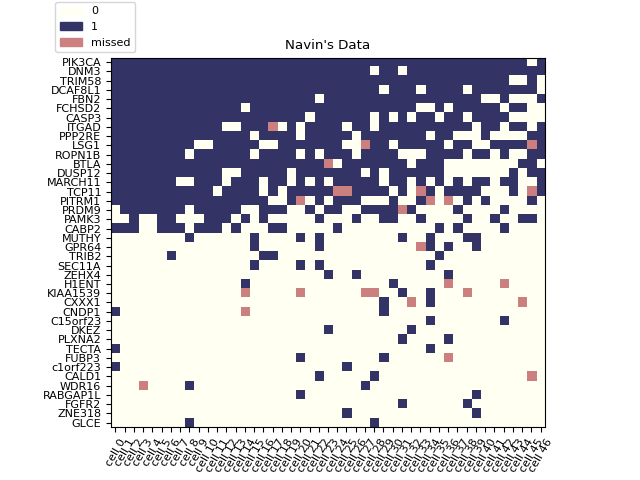
\includegraphics[width=0.67\textwidth]{img/dataset/r/Navin_Dm.png}
	\caption{درخت تصادفی اول}    
	\label{fig:ch_pm:pm1_T1}
\end{figure}

\subsection{پاسخی جدید}
تا به اینجا ما یک درخت فیلوژنی به عنوان پاسخ داریم که در این بخش می‌خواهیم با انجام تغییراتی بر روی آن به یک پاسخ جدید برسیم تا در گام‌های بعدی بتوانیم با مقایسه آن‌ها تصمیمات لازم را برای ادامه الگوریتم بگیریم. به همین منظور تقریبا مشابه با روش \cite{davis2016computing} به صورت \gls{pruneandreattach} قصد داریم تا درخت پاسخ فعلی را برای رسیدن به یک پاسخ دیگر تغییر دهیم. 
\begin{figure}[!ht]
	\centering 
	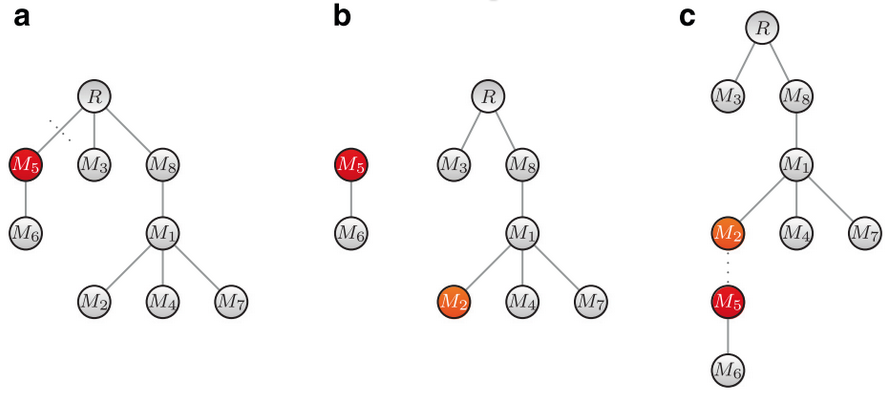
\includegraphics[width=0.9\textwidth]{img/chaps/pm/pruneandreattach}
	\caption{نحوه انجام کار روش \gls{pruneandreattach} \cite{davis2016computing}.}    
	\label{fig:ch_pm:pruneandreattach}
\end{figure}
در شکل \ref{fig:ch_pm:pruneandreattach} مثالی از این روش آورده شده است. در این شکل مطابق با قسمت \lr{a} یکی از نودهای درخت (به جز ریشه) انتخاب می‌شود (در اینجا نود \lr{$M_5$}) و اتصال از پدرش قطع می‌شود. در این حالت به دو درخت مشابه با شکل \lr{b} می‌رسیم. حال در درخت باقی مانده یک نود دیگر  (\lr{$M_2$}) به عنوان پدری جدید انتخاب می‌شود تا با این تغییر به درخت جدید شکل \lr{c} برسیم.
\\
در نتیجه با این تکنیک می‌توان به پاسخ‌های جدید رسید اما سوالی که باقی ماند این است که این دو نود چگونه باید انتخاب شوند؟ 
این دو انتخاب به صورت هوشمند توسط دو شبکه عمیق گرفته می‌شود. این شبکه‌ها که در اصل شبکه‌های \gls{reinforcementlearning} عمیق هستند، از پیش برای این منظور آموزش داده شده‌اند.
%\begin{equation}
%	\begin{aligned}
%		
%	\end{aligned}
%	T_{}
%	T_{i+1} = \text{Attach}(T_{i}, )
%\end{equation}
شبکه اول برای انتخاب محل برش (هرس) مورد استفاده قرار می‌گیرد و شبکه دوم با دریافت خروجی ××××××× دو درخت \gls{masterslave} مکان‌های مناسب برای بازاتصال را ارزش‌گزاری می‌کند. این دو شبکه در قسمت‌های \ref{sec:ch_pm:prune-network} و \ref{sec:ch_pm:reattach-network} به تفضیل شرح داده شده‌اند.

\subsection{مقایسه و ارزیابی پاسخ‌ها}
پس از اینکه از پاسخ فعلی به یک پاسخ جدید رسیدیم حال می‌توان کیفیت این دو پاسخ را باهم مقایسه کرد و پس از آن با توجه به امتیاز دو پاسخ در مورد پذیرش یا عدم پذیرش پاسخ جدید در برابر پاسخ فعلی تصمیم گرفت. این فرآیند شامل دو بخش اصلی است که در دو زیربخشی که در ادامه آمده است بیان شده‌اند.

\subsubsection{تبدیل درخت پاسخ به ماتریس}
برای ادامه روش پیشنهادی و مقایسات لازم است تا درخت پاسخ را به ماتریس $X$ تبدیل کنیم که قابل بررسی با داده‌های مشاهده شده $D$ باشد. ماتریس $X$ مشابه با ماتریس  $D$ متشکل از مقادیر $0$ و $1$ خواهد بود که به عنوان مثال $X_{i,j}=1$ به این معنی است که طبق درخت $T$ در سلول $i$ جهش $j$ مشاهده نشده است.
ما هر درخت $T$ را می‌توانیم با مقادیر مختلفی از $\sigma$ و $\wp$ مزین کنیم و به ماتریس‌های مختلفی برسیم. اما در نهایت مهمترین پارامترها که بیشترین امتیاز را برای درخت ما بوجود می‌آورند مطلوب ما خواهند بود و ماتریس متناظر با آن حالت را $X$ می‌نامیم و به مراحل بعدی برای محاسبات انتقال می‌دهیم.
در نتیجه کار ما در این بخش این خواهد بود که به ازای درخت دلخواه $T$ بتوانیم بهترین $\sigma$ و $\wp$ را بدست آوریم و از روی آن‌ها ماتریس متناظر $X$ را بدست آوریم.
از پیش با بررسی \glspl{cnp} در بخش 	\ref{sec:ch_pm:L} به $\mathcal{L}$ رسیده‌ایم که مشخص می‌کند چه جهش‌هایی پتانسیل حذف را دارند و در این بخش زمان استفاده از این اطلاعات است.
در ادامه ماتریس $B$ را به صورت رابطه \ref{eq:ch_pm:iB} تعریف می‌کنیم که برای انتخاب بهینه $\sigma$ مورد استفاده قرار خواهد گرفت.
 \begin{equation}
	B_{i,j} = 
	\begin{cases}
		1 		  &\qquad \text{\lr{if}} \quad \text{$i=j$ یا $i$ یکی از نوادگان $j$ باشد که در $\mathcal{L}$ نباشد} \\
		x 	 	  &\qquad \text{\lr{if}} \quad \text{$i$ یکی از نوادگان $j$ باشد و همچنین در $\mathcal{L}$ باشد} \\
		0 	       &\qquad \text{\lr{if}} \quad \text{در صورتی که دو مورد بالایی نباشد}
	\end{cases}
	\label{eq:ch_pm:iB}
\end{equation}
در رابطه بیان شده $x$ به معنای این است که هم می‌تواند مقدار $0$ و هم مقدار $1$ را داشته باشد.\\
حال می‌توانیم برای هر سلول (نمونه) $c_i$ در ماتریس مشاهده شده $D$ امتیاز اتصال را در هر قسمت از درخت $T$ حساب می‌کنیم که از طریق رابطه \ref{eq:ch_pm:score_B} بدست می‌آید.
\begin{equation}
	S(c_i, T, k) = \prod_{j=0}^{M}P(D_{i,j}|B_{j,k}) 
	\label{eq:ch_pm:score_B}
\end{equation}
در این رابطه $S(c_i, T, k)$ برابر امتیاز اتصال نمونه $i$ در درخت $T$ در مکان ژن (جهش) $k$ است.
ناگفته نماند که،
\begin{equation}
	P(D=1|B =x) = 1-\beta, \qquad P(D=0|B=x) = 1-\alpha
	\label{eq:ch_pm:score_p_x}
\end{equation}
بنابرین به ازای هر $x$ ما دو حالت را می‌توانیم داشته باشیم که آن‌ها همان پذیرش یا عدم پذیرش حذف جهش‌های در مجموعه $\mathcal{L}$ است. برای اینکه بهترین $\wp$ را داشته باشیم باید بتوانیم این امتیازاتی که با پذیرش‌های مختلف $x$ بدست می‌آیند را به ازای تمام نمونه‌های در دسترس ثبت و بررسی کنیم.
برای این منظور رابطه \ref{eq:ch_pm:iB} را به صورت رابطه \ref{eq:ch_pm:B} بازنویسی می‌کنیم.
 \begin{equation}
	B_{i,j} = 
	\begin{cases}
		1 		  &\qquad \text{\lr{if}} \quad \text{اگر $i$ یکی از نوادگان $j$ باشد که در $\mathcal{L}$ نباشد} \\
		x_{i}^{\text{\lr{dist($i$,$j$)}}} &\qquad \text{\lr{if}} \quad \text{اگر $i$ یکی از نوادگان $j$ باشد و همچنین در $\mathcal{L}$ باشد} \\
		0 	       &\qquad \text{\lr{if}} \quad \text{در صورتی که دو مورد قبلی نباشد}
	\end{cases}
	\label{eq:ch_pm:B}
\end{equation}
همان‌گونه که در این رابطه بیان شده همچنان مقادیر نامشخص وجود دارد. برای مشخص کردن این مقادیر نامشخص از $\wp$ استفاده می‌کنیم. $\wp$ یک لیست به طول تعداد ژن‌هایی است که در مجموعه $\mathcal{L}$ قرار دارند. نتیجه اعمال $\wp$ بر  $B$ ماتریس $A$ را نتیجه خواهد داد که به صورت زیر تعریف می‌شود.
\begin{equation}
	A_{i,j} = 
	\begin{cases}
		1 &\qquad \text{\lr{if}} \quad \text{$B_{i,j}=1$ یا $\wp_i<\text{\lr{dist($i$,$j$)}}$} \\
		0 &\qquad \text{\lr{if}} \quad \text{شرط بالا درست نباشد}
	\end{cases}
	\label{eq:ch_pm:A}
\end{equation}
این مقادیر نامشخص که در اتصال به ژن $i$ و نوادگان آن در درخت مشخص شده‌اند با توجه به فاصله تعیین شده از این ژن $i$ برای نوادگان حذف خواهد شد که این فاصله در $\wp_i$ مشخص شده است. پس حال با تعیین مقادیر بردار $\wp$ می‌توانیم بهترین $B$ نامعلوم را به $A$ معلوم تبدیل کنیم.
به رابطه \ref{eq:ch_pm:score_B} توجه کنید. این رابطه امتیاز اتصال نمونه $i$ را به مکان $k$ در درخت بیان می‌کند. ما به دنبال محلی هستیم که ضمیمه کردن نمونه به آن محل بالاترین امتیاز را بدست آورد. بنابرین $\sigma$ را به صورت یک بردار به طول $N$ (تعداد نمونه‌ها) تعریف می‌کنیم به طوری که شماره اندیس $i$ در آن متناظر با $i$امین نمونه در ماتریس $D$ باشد و مقداری که در آن خانه از $\sigma$ قرار می‌گیرد برابر با شماره یکی از ستون‌های ماتریس $A$ باشد که نشان‌دهنده بهترین محلی است که در درخت $T$ می‌تواند به آن ضمیمه شود.
حال می‌توانیم جایگاه هر اتصال به درخت را که بالاترین امتیاز را به ارمغان می‌آورد مشخص کنیم و پس از آن به تبدیل درخت $T$ به ماتریس $X$ بپردازیم.
\begin{equation}
	\begin{aligned}
		S(c_i, T) &= \max_{k \in \{0 \dots M\}} S(c_i, T, k) \\
		&= \max_{j^*} \left( \prod_{k=0}^{M}P(D_{i,k}|A_{k,j^*})\right) = S(c_i, T, \sigma_i)
	\end{aligned}
	\label{eq:ch_pm:score_attach}
\end{equation}
رابطه \ref{eq:ch_pm:score_attach} همان‌طور که مشاهده می‌شود به راحتی قابل حل می‌باشد و نمونه‌ها مستقل از هم هستند و می‌توانند به درخت اتصال یابند اما ما تا به اینجا بهترین $\sigma$ را به ازای یک $\wp$ یافته‌ایم. آیا مقدار $\wp$ نیز بهینه است؟
برای مشخص کردن مقدار بهینه $\wp$ برای درخت دلخواه $T$ از رابطه‌ای که در ادامه آمده است کمک می‌گیریم.
\begin{equation}
	\langle\hat{\wp}, \hat{\sigma}\rangle = \arg \max_{\wp, \sigma} \prod_{i=1}^{N}S(c_i, T)
	\label{eq:ch_pm:T_score}
\end{equation}
در واقع این مقادیر $\wp$ باید به گونه‌ای انتخاب شوند تا مجموع امتیازات همه اتصالات به درخت در حالت بیشینه خود باشد که برابر با امتیاز درخت می‌شود که در این حالت به $\hat{\wp}$ می‌رسیم که ماتریس $A$ حاصل از آن را $\hat{A}$ می‌نامیم. در نهایت که بهترین مقادیر به ازای درخت مشخص شدند پس می‌توان $X$ را به صورت رابطه \ref{eq:ch_pm:X} تشکیل داد.
\begin{equation}
	X_{i,j} = \hat{A}_{i, \hat{\sigma}_{j}}
	\label{eq:ch_pm:X}
\end{equation}







\subsection{یافتن جهش‌های با پتانسیل حذف}
\label{sec:ch_pm:L}

همان‌گونه که از ابتدا می‌دانیم ما به دنبال درخت فیلوژنی حقیقی داده‌های نویزی مشاهده شده $D$ هستیم. این درخت در این روش برابر با درختی است که،
\begin{itemize}
	\item نحوه قرارگیری ژن‌ها در ساختار درخت ($T$)
	\item محل‌هایی در درخت که جهش‌های قبلی در آن‌ها حذف می‌شوند ($\wp$)
	\item نحوه انتصاب نمونه‌های مشاهده شده به درخت ($\sigma$)
	\item و در نهایت پارامترهایی که برای مدل‌سازی خطای بوجود آمده در داده‌های در دسترس‌مان تعیین شده است ($\theta$)
\end{itemize}
به گونه‌ای انتخاب شوند که محتمل‌ترین حالت را برای مشاهده داده‌های $D$ بوجود آورند که در این حالت ما رابطه 
علت توضیحات مجدد این موارد به این دلیل است که این بخش مهمترین بخش در ساختار روش پیشنهادی اول است. 

\subsubsection{مقایسه پاسخ فعلی با پاسخ آرمانی}
پس از استخراج ماتریس مناسب از درخت می‌توان به ارزش‌گزاری و محاسبه \gls{likelihood} پرداخت. این عمل به صورت رابطه \ref{eq:ch_pm:pm1_likelihood} محاسبه می‌شود. 

\begin{equation}
	L: P(D|T,\sigma, \wp, \theta) = \prod_{n=1}^{n=N}\prod_{m=1}^{m=M}P(D_{nm}|X_{nm})
	\label{eq:ch_pm:pm1_likelihood}
\end{equation}
که $X$ برابر ماتریس بدست آمده از درخت $T$ با توجه به بردارهای $\sigma$ و $\wp$ است. این رابطه بیانگر احتمال مشاهده ماتریس داده ورودی $D$ در صورتی است که درخت فیلوژنی صحیح $T$ و پارامترهای حقیقی $\theta$ باشد که توسط بردارهای $\sigma$ و $\wp$ تثبیت شده است. هرچه این احتمال بالاتر باشد نمایانگر این است که درخت، پارامترها و بردارهای کنترلی ما بگونه‌ای انتخاب شده‌اند که محتمل‌ترین حالت برای مشاهده داده‌های ورودی ما هست و در این صورت بهترین پاسخ برای ما همان پاسخی خواهد بود که محتمل‌ترین باشد. از این رو با دانستن $\theta$ ما به دنبال $T$ای به همراه بردارهای مربوطه آن هستیم که پاسخ رابطه \label{eq:ch_pm:pm1_maxML} باشد.
\begin{equation}
	(T, \sigma, \wp)_{\text{\lr{ML}}} = \arg\max_{(T, \sigma, \wp)} P(D|T,\sigma, \wp, \theta)
	\label{eq:ch_pm:pm1_maxML}
\end{equation}
 اما همانگونه که می‌دانیم ما به دنبال بهترین درخت $T$ هستیم که $\sigma$ و $\wp$ در آن درخت برای ما اهمیت دارند. در واقع هر درخت $T$ دارای امتیاز $S(T)$ است که به صورت رابطه \label{eq:ch_pm:pm1_sT} تعریف می‌شود.
 \begin{equation}
 	S(T) = P(D|T,\sigma^*, \wp^*), \qquad \sigma^*=\arg\max_{\sigma}P(D|T,\sigma, \wp)
 	\label{eq:ch_pm:pm1_sT}
 \end{equation}

\subsection{پذیرش پاسخ‌های جدید و یافتن بهترین پاسخ}
در این مرحله ما دو پاسخ با امتیازهایشان در اختیار داریم که می‌توانیم برحسب آن‌ها برای ورود به \gls{iteration} بعد تصمیم‌گیری نماییم. این فرآیند توسط رابطه‌ای که در ادامه آمده است انجام می‌شود.
\begin{eqnarray}
	p_{\text{acc}} = \min\Bigg[1, \left(\frac{P(E=X_{i+1}|D, \theta)}{P(E=X_{i}|D, \theta)}\right)^{\rho^{-1}}\Bigg]
	 \label{eq:ch_pm:pm1_accepting} 
\end{eqnarray}
در رابطه \ref{eq:ch_pm:pm1_accepting}، اگر پاسخ جدید بهتر از پاسخ فعلی باشد بیان می‌کند که افزایش بهینگی در پاسخ جدید باعث می‌شود تا صورت کسر مقداری بیش از مخرج بگیرید که در این صورت $p_{\text{acc}}$ که برابر با احتمال پذیرش پاسخ جدید است، برابر $1$ خواهد شد که یعنی حتما پاسخ جدید به عنوان پاسخ پابرجا برای ورود به \gls{iteration} بعد در نظر گرفته می‌شود. اما اگر پاسخ جدید (درخت جدید) بهتر از پاسخ فعلی ارزیابی نشود ما آن را مستقیما رد نمی‌کنیم و به احتمالی کمتر از $1$ ممکن است آن را بپذیریم. دلیل این پذیرش جلوگیری از به دام افتادن الگوریتم در پاسخ‌مان در \gls{localmaxima} است. در شکل \label{fig:ch_pm:pm1_rho} تاثیر تغییر پارامتر $\rho$ در احتمال پذیرش پاسخ‌های جدیدی که مطلوب‌تر از پاسخ فعلی نیستند نمایش داده شده است.

\begin{figure}
	\centering
	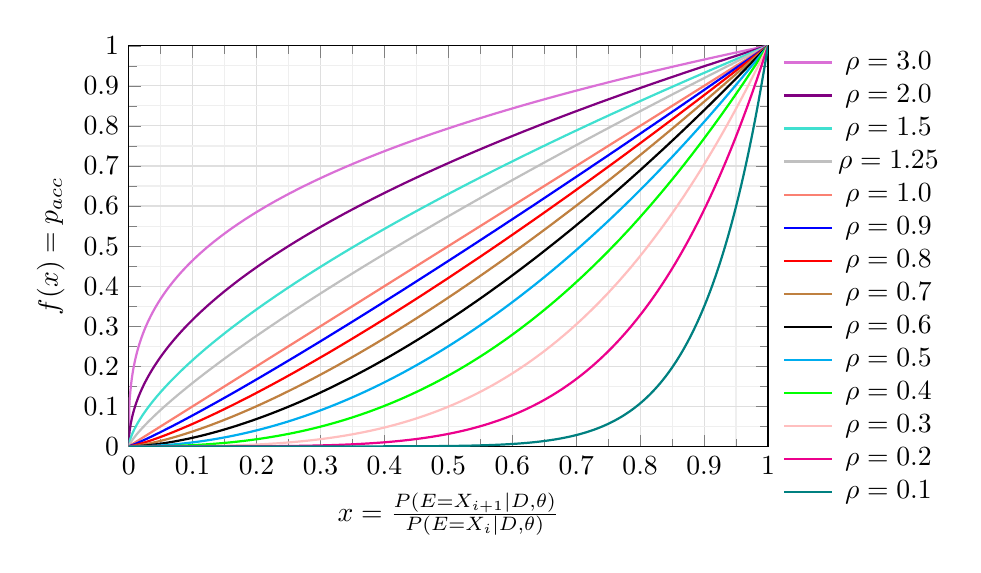
\begin{tikzpicture}
		\begin{axis}[xmin = 0, xmax = 1, ymin = 0, ymax = 1,
			xtick distance = 0.1, ytick distance = 0.1, grid = both, minor tick num = 1,
			major grid style = {lightgray!50}, minor grid style = {lightgray!25},
			width = 0.8\textwidth, height = 0.55\textwidth,
			xlabel = {$x=\frac{P(E=X_{i+1}|D, \theta)}{P(E=X_{i}|D, \theta)}$}, ylabel = {$f(x)=p_\text{acc}$},
			legend style={at={(1.01,1.015)}, draw=none, anchor=north west}]
			% Plot a function
			\addplot[domain = 0:1,samples = 1000,smooth,thick,Orchid,] {x^(3^-1)};
			\addplot[domain = 0:1,samples = 1000,smooth,thick,violet,] {x^(2^-1)};
			\addplot[domain = 0:1,samples = 1000,smooth,thick,Turquoise,] {x^(1.5^-1)};
			\addplot[domain = 0:1,samples = 1000,smooth,thick,Silver,] {x^(1.25^-1)};
			\addplot[domain = 0:1,samples = 100 ,smooth,thick,Salmon,] {x^(1.0^-1)};
			\addplot[domain = 0:1,samples = 100 ,smooth,thick,blue,] {x^(0.9^-1)};
			\addplot[domain = 0:1,samples = 100 ,smooth,thick,red,] {x^(0.8^-1)};
			\addplot[domain = 0:1,samples = 100 ,smooth,thick,brown,] {x^(0.7^-1)};
			\addplot[domain = 0:1,samples = 100 ,smooth,thick,black,] {x^(0.6^-1)};
			\addplot[domain = 0:1,samples = 100 ,smooth,thick,cyan,] {x^(0.5^-1)};
			\addplot[domain = 0:1,samples = 1000,smooth,thick,green,] {x^(0.4^-1)};
			\addplot[domain = 0:1,samples = 1000,smooth,thick,pink,] {x^(0.3^-1)};
			\addplot[domain = 0:1,samples = 1000,smooth,thick,magenta,] {x^(0.2^-1)};
			\addplot[domain = 0:1,samples = 1000,smooth,thick,teal,] {x^(0.1^-1)};
			% Legend
			\legend{$\rho=3.0$,$\rho=2.0$,$\rho=1.5$,$\rho=1.25$,$\rho=1.0$,$\rho=0.9$,$\rho=0.8$,$\rho=0.7$,$\rho=0.6$,$\rho=0.5$,$\rho=0.4$,$\rho=0.3$,$\rho=0.2$,$\rho=0.1$}
		\end{axis}
	\end{tikzpicture}
	\caption{نمودار تغییر احتمال پذیرش پاسخ جدید نامطلوب‌تر با توجه به مقدار پارامتر $\rho$.}
	\label{fig:ch_pm:pm1_rho}
\end{figure}

\newpage
\subsection{شبکه هرس‌کننده}
\label{sec:ch_pm:prune-network}

\subsection{شبکه بازاتصال‌کننده}
\label{sec:ch_pm:reattach-network}

\subsection{جمع‌بندی و نتیجه‌گیری}
روش پیشنهادی ما الگو گرفته شده از روش ارائه شده در مقاله سایت بود اما با این تفاوت که در آنجا فرض مکان‌های بی نهایت بود ولی ما فرض اسکارلت را جایگزین کردیم که در این بین چون فضای جست و جو بزرگتر شد در نتیجه مجبور شدیم نحوه برداشتن گام های خود را تغییر بدیم و هوشمندانه تر جلو برویم که در این فضای بزرگتر بتوانیم به جواب مناسب برسیم. در سایت برای رسیدن به درخت بهتر به دنبال تنظیم کردن پارامترهای خطا بود در حالی که ممکن بود با جواب واقعی فاصله داشته باشد اما چون بدنبال جواب با امتیاز بالا بود در نتیجه این پارامتری بودن و جست و جو برای مقادیر بهینه خطا در روش آن وجود داشت اما ما برای بهتر کردن امتیاز به جای تغییر پارامترهای خطا به ازای یک درخت جست و جوی ضمیمه کردن های مختلف سلول‌ها و لاس شدن جهش ها را جست و جو میکنیم.




\newpage

در این مقاله الگوریتم \lr{scarlet} معرفی شد که در آن به طور همزمان از \gls{snvv} (\lr{SNV}) و جهش‌های \gls{cnv} (\lr{CNA}) از داده‌های \gls{scs} برای استنباط فیلوژنی تومور استفاده شد. این الگوریتم، یک مدل تکاملی بر اساس در نظر گرفتن خطای ناشی از حذف جهش است که حذف جهش‌ها را محدود به مکان‌هایی می‌کند که شواهدی از حذف جهش‌های \gls{cnv} موجود باشد. مدلهای فیلوژنی \gls{losssupported}،  با استفاده از اطلاعات جهش‌های \gls{cnv} که به آسانی در داده‌های \gls{snvv} موجود است، نسب به مدل های \gls{dollo} یا فرض \gls{infinitesites}، \gls{conflict} کمتری در استنباط درخت فیلوژنی دارند. اگر چه به صورت طبیعی در داده‌های \gls{snvv} یک عدم قطعیت ذاتی در حضور یا عدم حضور جهش در سلول‌ها وجود دارد، اما کاهش میزان ابهام در استنباط فیلوژنی تومور منجر به افزایش \gls{accuracy} فیلوژنی استنباط شده است. در این مقاله نشان داده شد که فیلوژنی توموری استنباط شده برای بیماران مبتلا به سرطان روده از دقت و تکرارپذیری بیشتری برخوردار است و این الگوریتم در نهایت فیلوژنی‌هایی را استنباط کرد که در آن 3 حذف جهش رخ داده بود. البته این الگوریتم محدودیت‌های خاص خود را دارد. به عنوان مثال، این نوع پیاده‌سازی از الگوریتم اسکارلت مستلزم درخت \gls{cnv} به عنوان ورودی و میزان \gls{likelihood} هر یک از این درختان است. این رویکرد در مواقعی که تعداد مشخصی از تغییرات تعداد کپی وجود دارد قابل اجراست اما هنگامی که داده‌های \gls{scs} در مقیاس بزرگ انجام شود، به درختان زیادی از جهش‌های \gls{cnv} نیاز خواهد بود. 








%\section{روش پیشنهادی دوم}
%
%\subsection{مقدمه}
%
%\subsection{دادگان ورودی}
%
%\subsection{تبدیل داده‌ها به بردار ویژگی}
%
%\subsection{مدل‌سازی مساله}
%
%\subsubsection{معماری شبکه}
%
%\subsection{تابع هزینه}
%
%\subsection{اصلاح خطا و یافتن درخت جواب}

%\begin{table}[ht]
%	\caption{پارامترهای مدل ریاضی}
%	\label{tab:modelParameters}
%	\centering
%	\onehalfspacing
%	\begin{tabularx}{0.9\textwidth}{|r|X|}
%		\hline
%		$t_{ik}$			& زمان خدمت‌دهی به بیمار در مرحله $k$ام \\
%		\hline
%		$\tilde{t}_{ik}$	& زمان فاری خدمت‌دهی به بیمار در محله $k$ام \\
%		\hline
%		$t_{ik}^p$			& مقدار بدبینانه (حداکثر) برای زمان خدمت‌دهی به بیمار در مرحله $k$ام \\
%		\hline
%		$t_{ik}^m$			& محتمل‌ترین مقدار برای زمان خدمت‌دهی به بیمار در مرحله $k$ام \\
%		\hline
%		$t_{ik}^o$			& مقدار خوشبینانه (حداقل) برای زمان خدمت‌دهی به بیمار در مرحله $k$ام \\
%		\hline
%	\end{tabularx}
%\end{table}
%
%\begin{table}[ht]
%	\caption{متغیرهای مدل ریاضی}
%	\label{tab:modelVariables}
%	\centering
%	\onehalfspacing
%	\begin{tabularx}{0.9\textwidth}{|r|X|}
%		\hline
%		$X_{ild_{k}}$	& متغیر صفر-یک تخصیص بیمار به تخت/اتاق عمل\\
%		\hline
%		$S_{ild_{k}}$	& زمان شروع خدمت‌دهی به بیمار \\
%		\hline
%		$Y_{ijkl_{k}}$	& متغیر صفر-یک توالی بیماران \\
%		\hline
%		$V_{ni}$		& متغیر صفر-یک تخصیص جراح به بیمار‍‍ \\
%		\hline
%	\end{tabularx}
%\end{table}
